\documentclass[a4paper]{article}

\usepackage[utf8]{inputenc}
\usepackage{float}
\usepackage{graphicx}
\usepackage{subfig}

\begin{document}


\title{Lab 2: Raytracing}

\author{Karl Johan Andreasson \and Erik Fahlén}

\maketitle

\begin{figure}
    \centering
    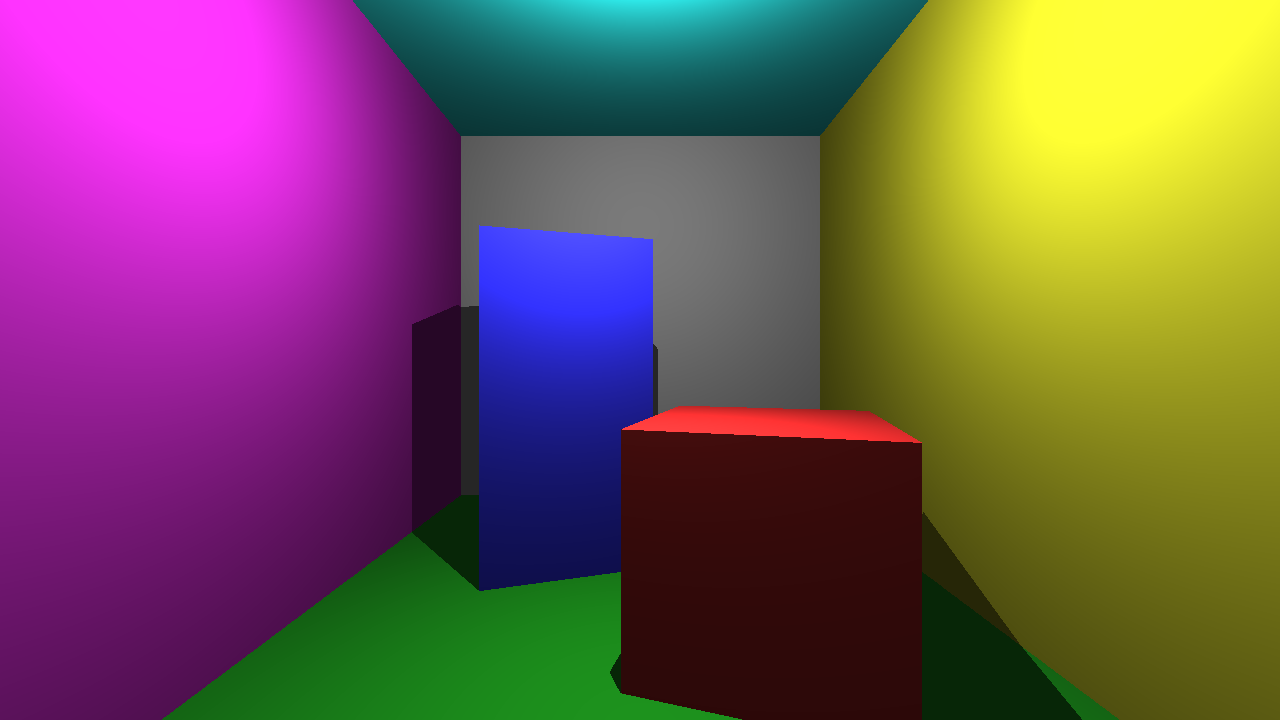
\includegraphics[width=10cm]{main720.png}
    \caption{The scene rendered.}
    \label{fig:main}
\end{figure}

\section{Introduction}
Computer graphics using raytracing is a common way of drawing very realistic and
pretty images using computers. However, it is not very useful for creating these
images in real time. To be able to create an image using raytracing in real time
requires some smart tricks and overall clever coding.

Raytracing is the process of shooting rays of and trace this path that the rays
travel and from this receive a very realistic looking image of the scene that is
to be rendered.

In this lab a scene constructed of a room with three walls, roof, floor and two
cubes all in different colors is drawn as seen in figure TODO!. Then shadowing
is implemented using the same manner; shooting rays from the lightsource and
discovering if the point is hidden (i.e. shadowed) or not.


\section{Implementation method}
In contrast to how we implemented the first lab where we worked individually and
then merged the two implementations into one, in this lab we worked together
throughout the implementing the lab. This worked really well and we could
discuss the implementation and math behind it and get a better understanding of
the math behind raytracing.

Implementing the raytracer of the scene given to us we started by attacking the
lab as described in the instructions. The instructions were well balanced in the
process of implementing a raytracer with the background of the assignment and
math to back it up together with the work to be implemented.

If the first lab was a bit too easy this lab was better structured in that the
first assignments was easier and then the difficulty increased as we progressed
through the lab.

The only place where we digressed from the lab instructions were when the
implementing of the shadows. In the lab the instructions was to shoot rays from
the light source towards the point and discovering if the point is the closest
intersection (and it should not be shadowed). We decided to shoot the rays from
the point being looked at towards the light source. This was really useful for
when the triangle intersections of the ray was really close to each other
because the comparison between the distance to the light source which usually is
quite a bit longer than the short distance to the other close intersection. The
main benefit of implementing the shadowing this way was that the rounding errors
present using floats could be ignored completely.

\section{Discussion}
In this lab the major problem was to really understand the math and how this
should be implemented to make sure the raytracer is as fast as possible to try
to make it work in real time.

We had some problems when trying to find the closest intersecting triangle. We
used the function vec3::length however this did not return the euclidean
distance but something else. The function that we ended up using was
glm::distance. This was according to our experience badly documented and we
basically had to guess what functions that were available to use. Acctually a
lot of the implementation time was used trying to figure out this very problem.

When the lab was completed we tried to make it faster as to render one frame
using a screen resolution of 1280x720 up to 23.5 seconds. We played around with
various optimization attempts and profiling of the code. We realized quickly
that the major bottleneck in the program was calculating the inverse of the
matrix to get the intersection of the ray and the triangle looked at currently.
We use the function glm::inverse to calculate this inverse hence we could not
optimize this any further without writing our own matrix inverse function. We
then discovered that the optimization flag O3 in g++ would provide an incredible
speedup and the same fram with a resolution of 1280x720 would now take around 0.5
seconds.

\section{Result}
The resulting raytracer works really well on our own machines, escpecially once
the optimization flag was set during compiling of the code. 

As demonstrated in figure \ref{fig:camera} the camera can be moved around and
the view are as expected from a pin-hole camera.

The light source can be moved around as well, as specified in the lab report. A
demonstration of this can be seen in figure \ref{fig:light}.

\begin{figure}[H]
    \centering
    \begin{minipage}{.5\textwidth}
        \centering
        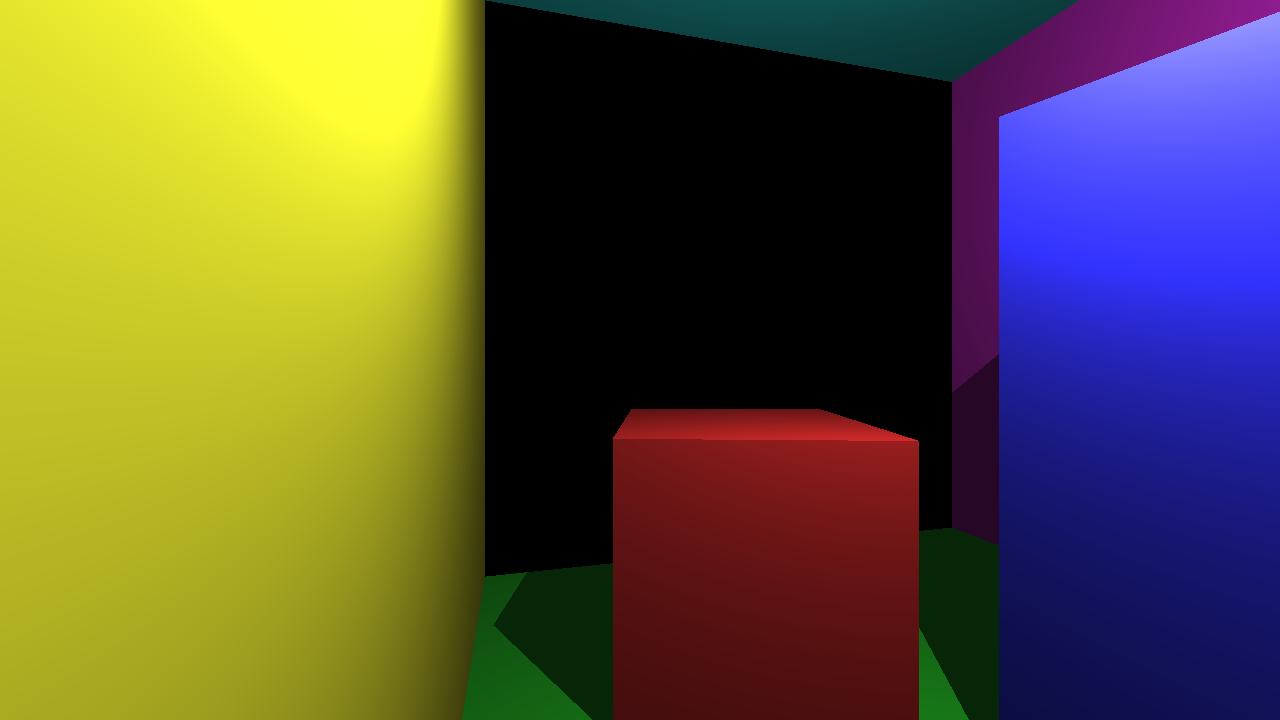
\includegraphics[width=4cm]{720ani0.png}
    \end{minipage}%
    \begin{minipage}{.5\textwidth}
        \centering
        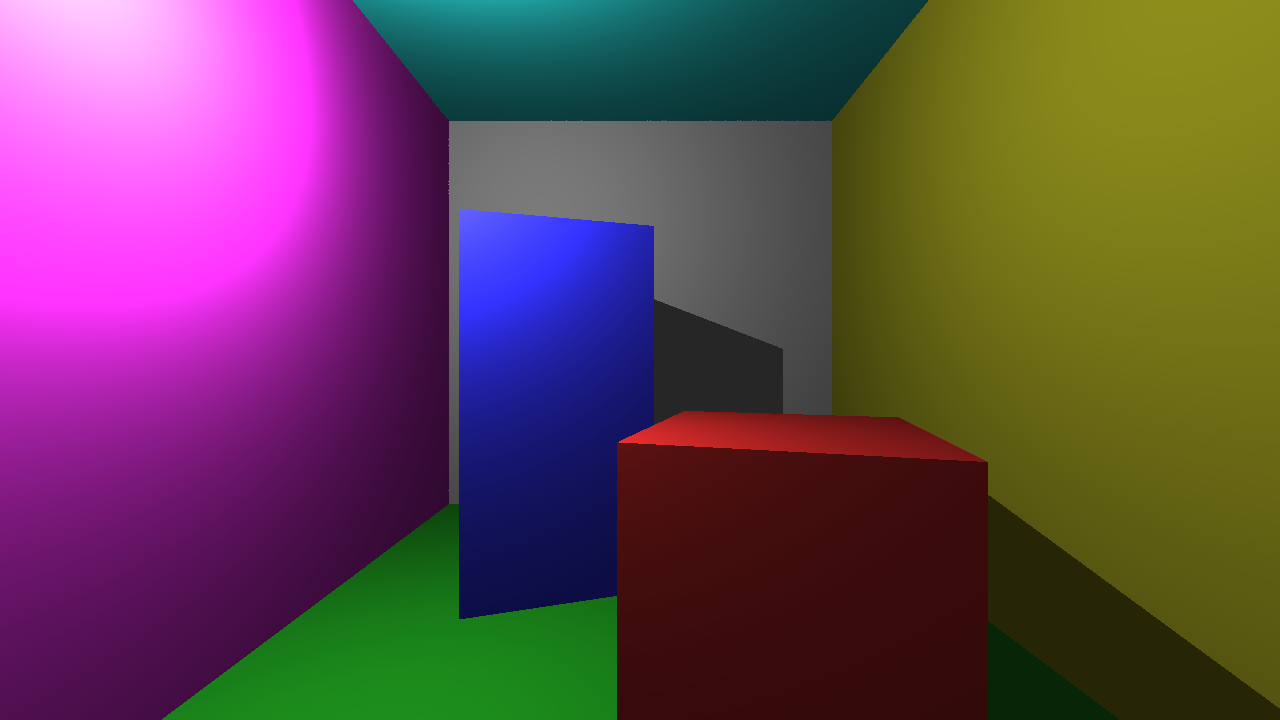
\includegraphics[width=4cm]{light0.png}
    \end{minipage}
\end{figure}

\begin{figure}[H]
    \centering
    \begin{minipage}{.5\textwidth}
        \centering
        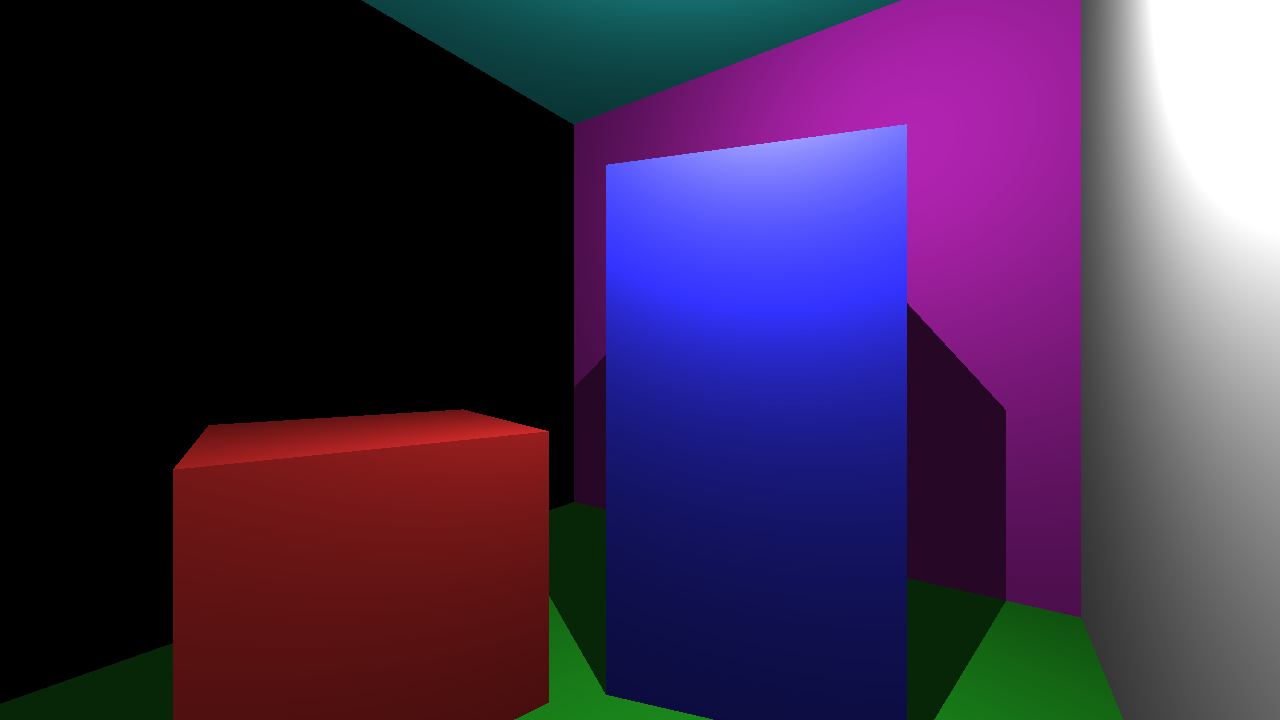
\includegraphics[width=4cm]{720ani1.png}
    \end{minipage}%
    \begin{minipage}{.5\textwidth}
        \centering
        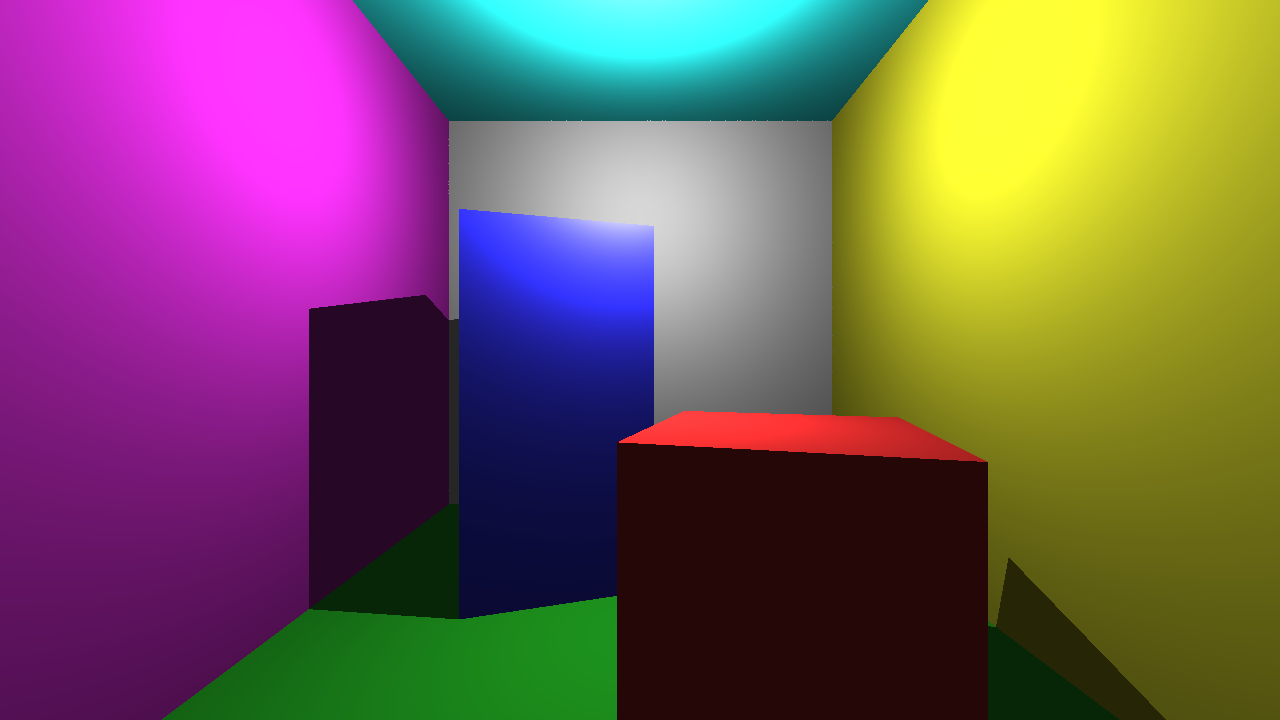
\includegraphics[width=4cm]{light1.png}
    \end{minipage}
\end{figure}

\begin{figure}[H]
    \centering
    \begin{minipage}{.5\textwidth}
        \centering
        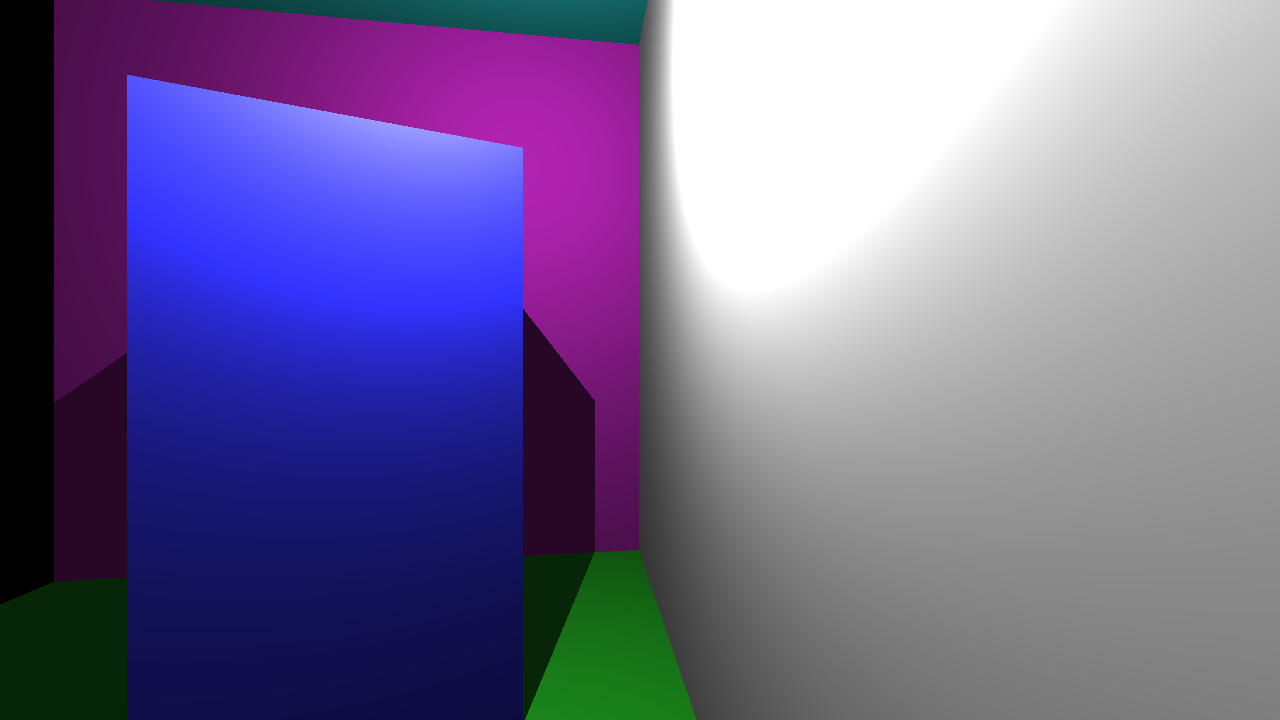
\includegraphics[width=4cm]{720ani2.png}
        \captionof{figure}{\\Moving the camera around.}
        \label{fig:camera}
    \end{minipage}%
    \begin{minipage}{.5\textwidth}
        \centering
        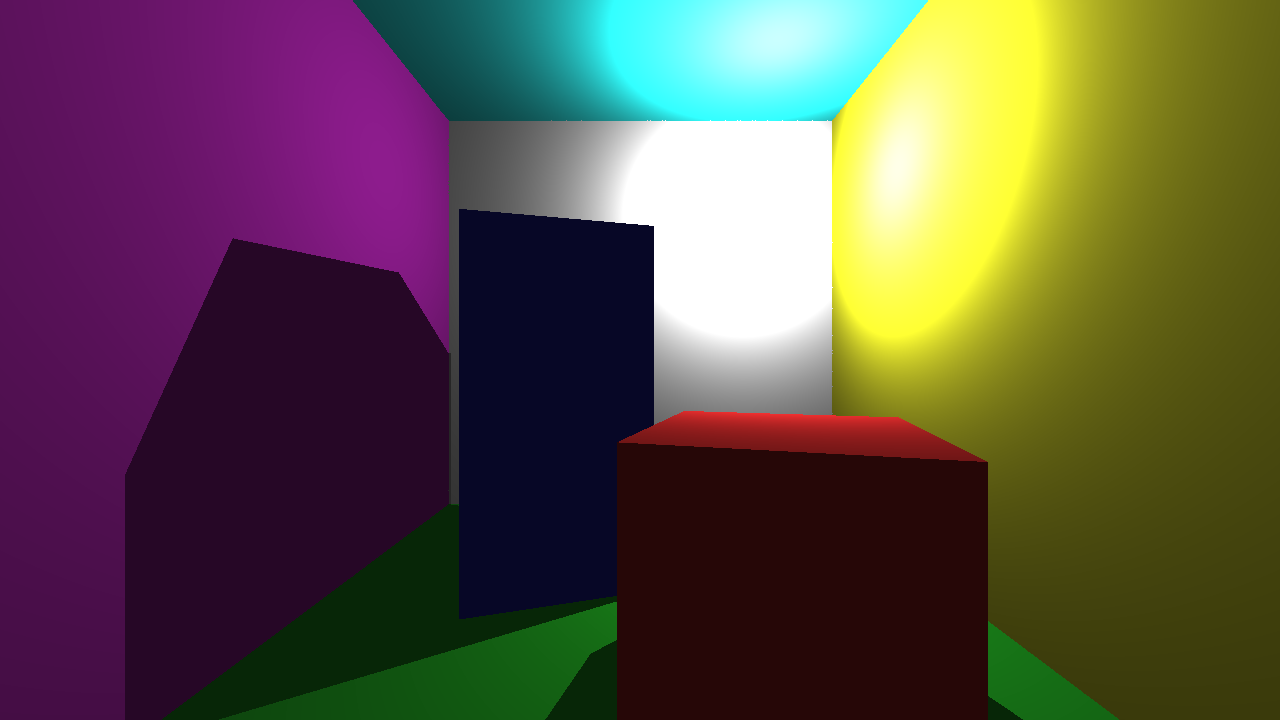
\includegraphics[width=4cm]{light2.png}
        \captionof{figure}{\\Moving the light source around.}
        \label{fig:light}
    \end{minipage}
\end{figure}

\end{document}
